\section{Technique}
%
To add path merging to SPF, we first pre-compute static summaries of arbitrary code regions with more than one execution
path and methods.
%
To bound the set of code regions we analyze, we start by specifying a method $M$ in a configuration file.
%
Next, we construct a set containing only the class $C$ that contains $M$.
%
We then get another set of classes, $C'$,
such that every class in $C'$ has atleast one method that was called by a method in a class in $C$.
%
This step which goes from $C$ to $C'$ discovers all the classes at a call depth of 1 from $C$.
%
We continue this method discovery process up to a call depth of 2.
%
While we can increase the call depth in our method discovery process, we found that summarizing
arbitrary code regions more than 2 calls deep did not lead to practically useful region summaries.
%
After obtaining a list of methods, we computed static summaries of regions in these methods and method summaries as
explained in Section \ref{sec:static-analysis}.
%
To make use of region summaries in Symbolic PathFinder, we use an existing feature of SPF named \textit{listener}.
%
A listener is a method defined within SPF that is called for every bytecode instruction executed by SPF.
%
Java Ranger adds a path merging listener to SPF that, on every instruction, checks (1) if the instruction involves
checking a symbolic condition, and (2) if Java Ranger has a pre-computed static summary that begins at that
instruction\rq s bytecode offset.
%
If both of these conditions are satisfied, Java Ranger instantiates the multi-path region summary by reading inputs from
and writing outputs to the stack and the heap.
%
It then conjuncts the instantiated region summary with the path condition and resumes symbolic execution at the
bytecode offset of the end of the region.
%
The instantiation of the region summary is performed as a sequence of transformations described below and summarized
in Figure~\ref{fig:overview}.
%
\begin{figure}[]
    \caption{Overview of transformations on Ranger IR to create and instantiate multi-path region summaries with higher-order regions}
    \label{fig:overview}
    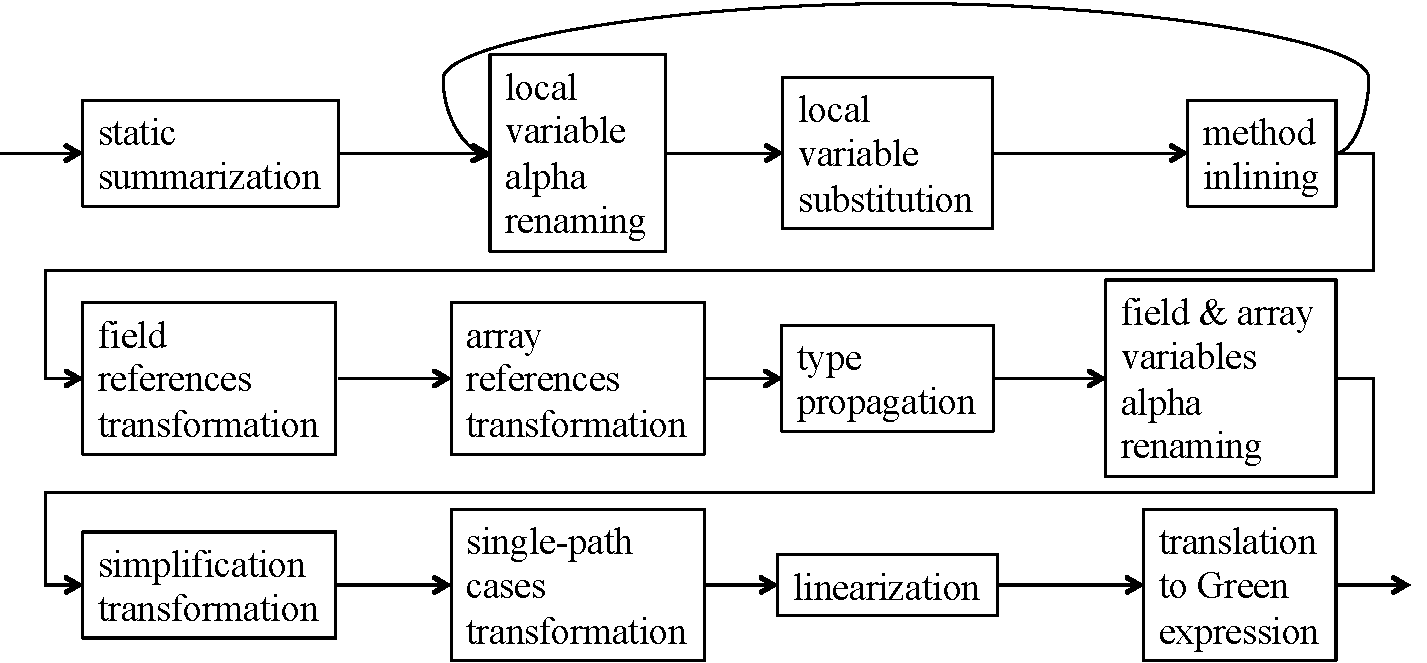
\includegraphics[width=\textwidth]{figures/overview.pdf}
\end{figure}
%
%
%\subsection{WALA-based analysis for veritesting}
%%
%Veritesting requires static construction of
%predicates of a multi-path region which represent changes to the path expression of the dynamic
%symbolic executor.
%%
%It also requires construction of a control-flow graph of method bodies
%from Java bytecode and finding exit points of the region, which in turn
%requires creation of a control-flow graph of the region.
%%
%Implementing veritesting is made simpler by using a static single
%assignment~(SSA)~\cite{ssa} representation of the multi-path region.
%%
%Using an SSA form allows us to use the $\phi$-expressions created by the
%SSA form and translate them into points at the end of the veritesting
%region where updates to system state along different paths in the region
%can be merged.
%%
%\mike{MWW: Vaibhav please update to describe WALA}
%WALA~\cite{} is a static analysis framework for Java programs that
%has both these features, with
%ExceptionalUnitGraph~\cite{exceptionalunitgraph} and the Shimple
%IR~\cite{shimple}.
%%
%For simple regions with only one exit point, like the one presented in Listing~\ref{lst:v_ex}, we
%were able to use Soot to automate static construction of the predicate representing
%an update to the expression.
%%
%For doing this, we used nodes with more than one successor as the
%starting point, found the immediate post-dominator of the starting
%point, and traversed the control-flow graph on all sides of such branches.
%%
%During such a traversal, we constructed predicates representing the
%multi-path region, similar to the ones presented in
%Listing~\ref{lst:v_ex_smt2}.
%%
%As explained in Section~\ref{sec:exit_points}, including virtual
%function invocations in the construction of our predicates amplifies the
%benefits of veritesting even further.
%%
%We plan to automate this inclusion in the future using Soot.
%%
%Providing SPF with updates to be made to its symbolic store also
%requires Soot to maintain stack location information for variables.
%%
%We plan to automate SPF\rq s symbolic store updates using Soot in the
%future.
%%
%

\subsection{Representation of Static Regions}
\label{sec:static-analysis}
\vaibhav{assigned to Mike}
\mike{MWW: - we should provide an AST of the constraint language}

\subsection{Instantiation-time Transformations}
\textbf{Alpha Renaming}: assigned to Soha\\
\textbf{Local Variable Substitution}: assigned to Soha\\
\textbf{Higher-order Regions}: assigned to Soha\\
\textbf{Field References SSA form}: assigned to Vaibhav\\
\textbf{Array References SSA form}: assigned to Vaibhav\\
\textbf{Simplification of Ranger IR}: assigned to Vaibhav\\
\textbf{Single Path Cases}: assigned to Soha\\
\textbf{Linearization}: assigned to Mike or Soha (whoever grabs it first)\\
\textbf{Translation to Green}: assigned to Soha\\

\subsection{Checking Correctness}
\vaibhav{assigned to Vaibhav}

